\subsection{Rectas y Planos}
Un conjunto de puntos son llamados \textbf{colineales} si pertenecen a una misma recta, lo que puede ser verificado por la igualdad constituida entre las pendientes entre cada par. En álgebra lineal, también se puede verificar comprobando si el área del polígono formado entre los puntos es cero. Trivialmente, todo par de puntos en un plano son colineales, ya que forman una línea.\\

Dos rectas en un mismo plano son llamadas \textbf{coincidentes} si están constituidas por el mismo conjunto de puntos, \textbf{paralelas} si no tienen ningún punto en común (igual pendiente), \textbf{secantes} si solo se intersectam en un punto y \textbf{perpendiculares} si forman entre ellas ángulos rectos ($m_1 \cdot m_2 = -1$).\\

\subsubsection{Teorema de Thales}
Si dos o más \textbf{rectas paralelas} se intersectan por dos transversales, entonces las medidas de los segmentos determinados sobre las secantes son \textbf{proporcionales}.
\begin{center}
\colorbox{white}{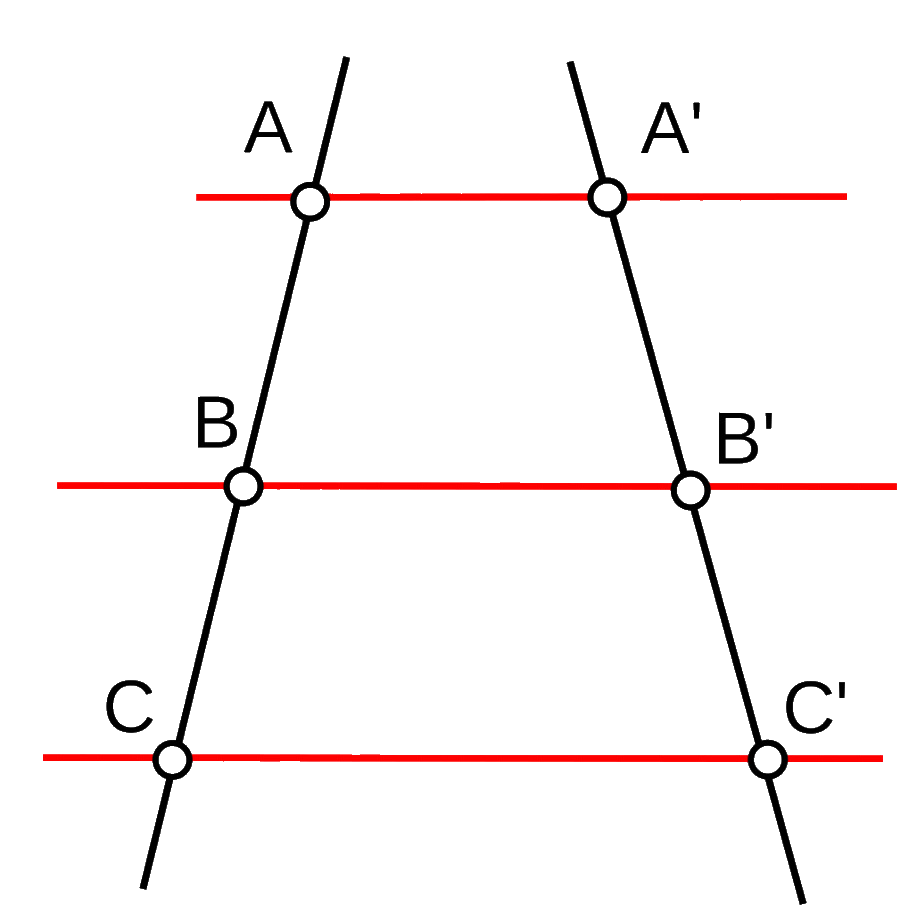
\includegraphics[width=0.5\columnwidth]{teoremathales.png}}
\end{center}
\subsubsection{Teorema Particular de Thales}
Establece que un segmento de recta paralelo a un lado de un triángulo y que corta a los otros dos, determina en estos últimos segmentos proporcionales. Es importamente mencionar de que el teorema es \textbf{recíproco}.
\begin{center}
    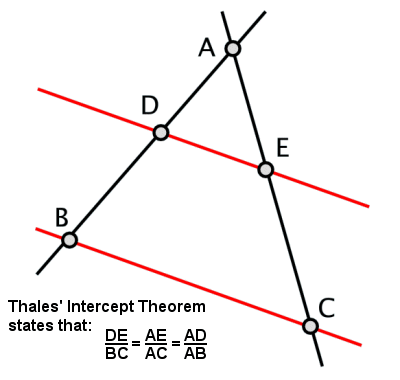
\includegraphics[width=0.8\columnwidth]{teoremathalesparticular.png}
\end{center}
\subsubsection{Ecuación Vectorial y Paramétrica}
Una recta puede ser expresada en la forma de una \textbf{ecuación vectorial} donde se encuentra definida por un punto de ella, y su dirección. Cualquier vector con la misma dirección (ángulo o pendiente) con respecto a la recta, es llamado \textbf{vector director} ($\vec{d}$), y asimismo un vector de un punto P perteneciente a la recta, es llamado \textbf{vector de posición} ($\vec{P_0}$).\\

De esta forma, la ecuación vectorial de la recta está dada por: \\
$\vec{p} = \vec{p_0} + \lambda\vec{d}$, donde $\lambda \in \mathbb{R}$ y $\vec{p}$ es un vector representando cualquier punto en la recta.

% Intuitivamente, esto significa de que a medida de que $\lambda$ cambia, este modifica la magnitud (por ponderación) de el vector dirección que después es ubicado en el plano por el vector posición.

% Una \textbf{ecuación paramétrica} define un grupo de cantidad como funciones de una o mas variables independientes, llamadas \textbf{parámetros}. Son comúnmente usadas para expresar las coordenadas de puntos que forman objetos geométricos como una curva o una superficie, en cuyo caso se llaman \textit{representaciones parámetricas}.\\

Al resolver la forma general tal que quede expresada en un solo vector, se pueden generar un conjunto de \textbf{ecuaciones paramétricas} (con parámetro $\lambda$) que determinan la recta a través de cada una de sus componentes (como se expresan en el vector resultante).\\

En el plano, la ecuación vectorial puede ser expresada como:

\begin{equation*}
(x, y) = (x_0, y_0) + \lambda(d_x,d_y) \text{ con } \lambda \in \mathbb{R}
\end{equation*}

Y paramétricamente:
\begin{equation*}
    \begin{rcases}
      x = x_0 + \lambda d_x \\
      y = y_0 + \lambda d_y
    \end{rcases}
    \lambda \in \mathbb{R}
    \end{equation*}
Teniendo una ecuación paramétrica, podemos despejar el parámetro ($\lambda$) en cada uno, y despues igualar las expresiones equivalentes del parámetro para obtener una \textbf{ecuación continua} de la forma:
\begin{equation*}
\begin{split}
    \lambda &= \frac{x - x_0}{d_x}\\
    \lambda &= \frac{y - y_0}{d_y}\\
    \frac{x-x_0}{d_x} &= \frac{y-y_0}{d_y}
\end{split}
\end{equation*}